\section{Our Research} 

\subsection{Our Motivation}

It corresponds to O'Reillys motivations \cite{o1998six}.

O'Reilly presents what he thinks as biologically plausible. In the end of this review we provide citations from this article which shortly explain the most important concepts of NN design. 

Article also contains interesting references to several experiments. It also presents the Leabra model (PhD thesis of O'Reilly) which is presented as a base model for other NN which can be derived from Leabra. The question how to merge the proposed principles is dicussed, especially the case of competiveness and distributed representation. 

\paragraph{Biological realism.} Moreover, computational mechanisms that violate
known biological properties should not be relied upon. 

A criticism of back-propagation is that it is neurally implausible (and hard to implement in hardware) because it requires all the connections to be used backward and it requires the units to use different input-output functions for the forward and backward passes \cite{hinton1988learning}.

\paragraph{Distributed representations.} A distributed representation
uses multiple active neuron-like processing units to encode
information (as opposed to a single unit, localist represen-
tation), and the same unit can participate in multiple repre-
sentations. Each unit in a distributed representation can be
thought of as representing a single feature, with information
being encoded by particular combinations of such features \cite{hinton1988learning}.


\paragraph{Inhibitory competition.} Inhibitory competition arises when mutual
inhibition among a set of units (i.e. as mediated by in-
hibitory interneurons) prevents all but a subset of them
from becoming active at a time.  Furthermore, most learn-
ing mechanisms (including those discussed later) are
affected by this selection process such that only the selected
representations are refined over time through learning, re-
sulting in an effective differentiation and distribution of
representations. More generally, it seems as though the world can be usefully
represented in terms of a large number of categories with a
large number of exemplars per category (animals, furniture,
trees, etc.) \cite{hinton1988learning}. 

\paragraph{Bidirectional activation propagation (interactivity).} They showed that
interactivity could explain the counterintuitive finding that
higher-level word processing can influence lower-level letter
perception. More recently, Vecera and O’Reilly showed
that bidirectional constraint satisfaction can model people’s
ability to resolve ambiguous visual inputs in favor of familiar
versus novel objects \cite{hinton1988learning}. 

\paragraph{Error-driven task learning.} Error-driven learning (also called ‘supervised’ learning) is
important for shaping representations according to task de-
mands by learning to minimize the difference (i.e. the error)
between a desired outcome and what the network actually
produced \cite{hinton1988learning}. 

\paragraph{Hebbian model learning.} That something like correlational structure is important.
Hebbian learning mechanisms represent this correlational
structure, encoding the extent to which different things co-
occur in the environment \cite{hinton1988learning}.


\paragraph{Hebbian nature.}

TODO: Read and cite from Hebbs's original article (Hebb, D.O. (1949). The organization of behavior. New York: Wiley \& Sons). 

(Wiki) Hebbian theory is a scientific theory in biological neuroscience which explains the adaptation of neurons in the brain during the learning process. It describes a basic mechanism for synaptic plasticity wherein an increase in synaptic efficacy arises from the presynaptic cell's repeated and persistent stimulation of the postsynaptic cell. Introduced by Donald Hebb in 1949, it is also called Hebb's rule, Hebb's postulate, and cell assembly theory, and states:

    "Let us assume that the persistence or repetition of a reverberatory activity (or "trace") tends to induce lasting cellular changes that add to its stability. When an axon of cell A is near enough to excite a cell B and repeatedly or persistently takes part in firing it, some growth process or metabolic change takes place in one or both cells such that A's efficiency, as one of the cells firing B, is increased."

The theory is often summarized as "Cells that fire together, wire together.".[1] It attempts to explain "associative learning", in which simultaneous activation of cells leads to pronounced increases in synaptic strength between those cells. Such learning is known as Hebbian learning.

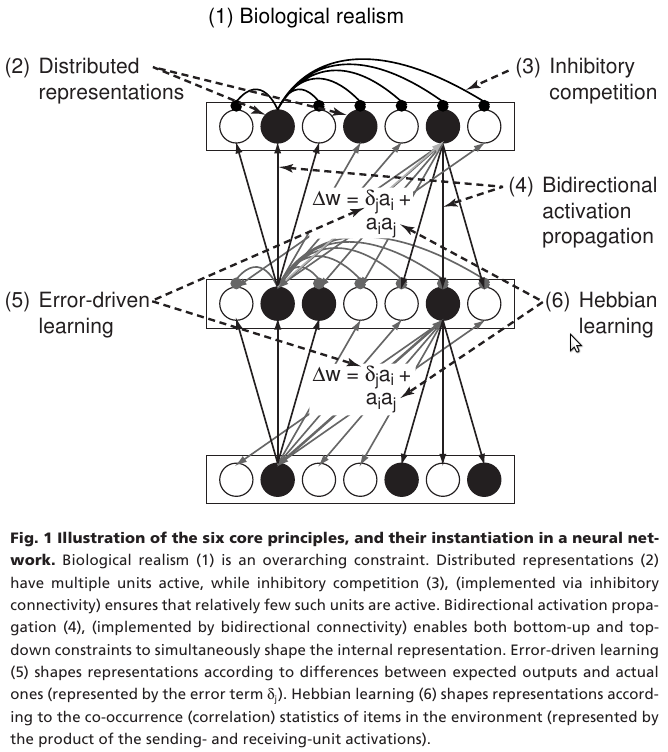
\includegraphics[width=12cm]{img/bio_plausability_o1998six.png}



\subsection{Considered modifications}
Viacero z prezentovaných modifikácií boli aplikované na iné typy neurónových sietí. My sme sa zaoberali aplikáciami na Generec, analyzovali sme ich konvergenciu a aplikovali ich na štandardnej sade úloh. 

\subsubsection{Regression} 

\textit{Regression} means that, after one pass around the loop, instead of setting the activity of a visible unit, $i$, to be equal to its current total input, $x_i(2)$, as determined by 
$$x_j = \sum_i y_iw_{ji} - \theta_j,$$
we set its activity to be 
$$y_i(2) = \lambda y_i(0) + (1-\lambda)x_i(2)$$
where the regression, $\lambda$, is close to 1. Using high regression ensures that the visible units only change state slightly so that when the new visible vector is sent around the loop again on the second pass, it has very similar effects to the first pass \cite{hinton1988learning}.

\subsubsection{Ballard}
Merging several closed loops of recirculation. 

Since the same learning rule is used for both visivle and hidden units, there is no problem in applying it to systems in which some units are the visible units of one module and the hidden units of another \cite{hinton1988learning}. 

We do not have a formal analysis \cite{hinton1988learning}.
%D.H. Ballard Proc. American Association for Artificial Intelligence, Seatle, WA, 1987

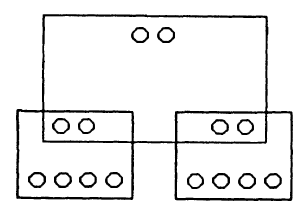
\includegraphics[width=8cm]{img/ballard.png}

\subsubsection{Dropout}
When a large feedforward neural network is trained on a small training set,
it typically performs poorly on held-out test data. This \emph{overfitting} is greatly
reduced by randomly omitting half of the feature detectors on each training
case. This prevents complex co-adaptations in which a feature detector is only
helpful in the context of several other specific feature detectors. Instead, each
neuron learns to detect a feature that is generally helpful for producing the
correct answer given the combinatorially large variety of internal contexts in
which it must operate. Random \emph{dropout} gives big improvements on many
benchmark tasks and sets new records for speech and object recognition.
 \cite{hinton2012improving} (Abstract copied). 
 
 TODO: Read the article. 
 
Conceptually the idea is simple. In each activation phase turn off randomly a half of all hidden neurons. This should restrict coadaptation of neurons. It a desired quality as we want from each unit to represent a different feature. If the units can coadapt then it might occur that more units represent the same feature. 

\subsubsection{Deep architectures} 
TODO  \cite{bengio2009learning}.

\subsection{Comparison}
TODO
